\documentclass{beamer}
\usetheme{Madrid}
\usecolortheme{default}
\usepackage[utf8]{inputenc}
\usepackage{amsmath, amssymb, bm}
\usepackage{graphicx}
\usepackage{booktabs}
\usepackage{hyperref}

% --------------------
% Metadata
% --------------------
\title[World Trade Overview]{World Trade -- An Overview\\\small{Krugman, Obstfeld \& Melitz, 12th Edition (Chapter 2)}}
\author{Prepared by: Macro/Trade Lecture Notes}
\date{\today}

% --------------------
% Document
% --------------------
\begin{document}

% Title Slide
\begin{frame}
  \titlepage
\end{frame}

% Agenda
\begin{frame}{Agenda}
\tableofcontents
\end{frame}

\section{Learning Objectives}
\begin{frame}{Learning Objectives}
After this lecture, you should be able to:
\begin{itemize}
  \item Describe how the value of trade between any two countries depends on the size of these countries’ economies and explain the reasons for that relationship.

 % \item State and interpret the gravity model of trade and its parameters.
  \item Describe why distance and borders still matter for trade.
  \item Summarize the two ages of globalization and their reversals.
  \item Discuss how the composition of world trade has evolved (goods, services, GVCs).
  \item Connect empirical patterns to policy and macroeconomic performance.
\end{itemize}
\end{frame}

\section{Empirical Landscape}
\begin{frame}{Stylized Facts of World Trade}
\begin{itemize}
  \item Trade is concentrated among large economies; small and proximate partners trade disproportionately with each other.
  \item The share of trade in world GDP rose sharply post-1945, with interruptions around major crises.\\
  
  \item Bilateral trade is highly correlated with partners' GDP and negatively related to distance.\\
  
 \item More than 30 percent of world output is sold across national borders.\\
 \begin{itemize}
\item World trade in goods and services exceeded $\$25$ trillion in 2019.
 \end{itemize}
\end{itemize}
\end{frame}

\begin{frame}{Stylized Facts of World Trade Cont'd}

\begin{figure}[ht]
        \centering
        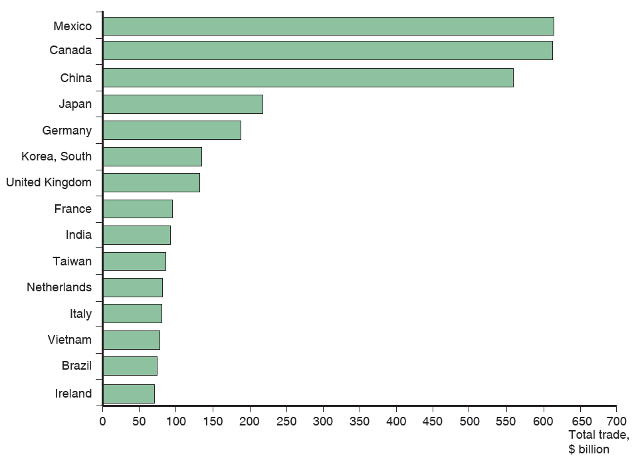
\includegraphics[width=0.6\linewidth]{Figure1.png}
        \caption{Total U.S. Trade with Major Partners, 2019}
        \label{fig:example}
\end{figure}
\begin{itemize}
\item U.S. trade is measured as the sum of imports and exports - mostly with 15 major partners.

\end{itemize}
\end{frame}

\begin{frame}{Stylized Facts of World Trade Cont'd}
\begin{itemize}

\item Figure 2-1 shows the total value of trade in goods exports plus imports between the United States and its top 15 trading partners in 2019.
\begin{itemize}

\item The largest 15 trading partners with the United States accounted for 75 percent of the value of U.S. trade.\\
\end{itemize}
\item The five largest trading partners with the United States in 2019 were Mexico, Canada, China, Japan, and Germany.
  
\end{itemize}
\end{frame}







\section{Gravity Model}
\begin{frame}{Size Matters,  The Gravity Model}
\begin{itemize}
\item Three of the top 15 U.S. trading partners are European nations: Germany, the United Kingdom, and France.
\item Why does the United States trade more with these European countries than with others?
\begin{itemize}
\item These three countries have the largest gross domestic product (G D P), the value of goods and services produced in an economy, in Europe.
\end{itemize}
\end{itemize}




A parsimonious empirical relationship:
\begin{equation*}
T_{ij} = A\, \frac{Y_i^{\alpha} Y_j^{\beta}}{D_{ij}^{\gamma}} \times \exp\{\bm{z}_{ij}'\delta\},
\end{equation*}
where $T_{ij}$ is trade from $i$ to $j$, $Y_i, Y_j$ are GDPs, $D_{ij}$ is distance, and $\bm{z}_{ij}$ contains frictions (common language, border, trade agreement, etc.).
\end{frame}

\begin{frame}{Log-Linear Specification and Interpretation}
Taking logs:
\begin{equation*}
\ln T_{ij} = c + \alpha \ln Y_i + \beta \ln Y_j - \gamma \ln D_{ij} + \bm{z}_{ij}'\delta + \varepsilon_{ij}.
\end{equation*}
\begin{itemize}
  \item $\alpha,\beta \approx 1$: trade proportional to size.
  \item $\gamma > 0$: distance elasticity; often near unity in estimates.
  \item Elements of $\bm{z}_{ij}$: common language ($+$), border ($-$), FTA ($+$), currency union ($+$).
\end{itemize}
\end{frame}

\begin{frame}{Structural Gravity (Sketch)}
Under CES preferences and iceberg costs $\tau_{ij} \ge 1$:
\begin{equation*}
X_{ij} = \frac{Y_i\,E_j}{Y^W} \left(\frac{\tau_{ij}}{\Pi_i P_j}\right)^{1-\sigma},
\end{equation*}
where $X_{ij}$ is expenditure of $j$ on goods from $i$, $\sigma>1$ is elasticity of substitution, $\Pi_i$ and $P_j$ are multilateral resistance terms, and $Y^W$ world income.
\begin{itemize}
  \item Captures general equilibrium: bilateral trade depends on \emph{all} trade costs via $\Pi_i, P_j$.
  \item Empirically implemented with exporter and importer fixed effects.
\end{itemize}
\end{frame}

\section{Distance and Borders}
\begin{frame}{Why Distance Still Matters}
\begin{itemize}
  \item Transportation and logistics: bulky/perishable goods face non-trivial costs.
  \item Information and trust: proximity reduces uncertainty and search costs.
  \item Regional production networks: NAFTA/USMCA, EU, ASEAN reinforce neighborhood trade.
\end{itemize}
\end{frame}

\begin{frame}{Beyond Tariffs: Border Effects}
\begin{itemize}
  \item Legal, regulatory, standards, and customs procedures.
  \item Currency and financial frictions; exchange rate risk.
  \item Culture and language; business practices and contract enforcement.
\end{itemize}
\vspace{0.5em}
Empirically, border dummies are large in gravity regressions, even holding distance constant.
\end{frame}

\section{Globalization in Two Waves}
\begin{frame}{First Age (pre-1914)}
\begin{itemize}
  \item Technology: steamships, railways, telegraph; sharp drop in trade costs.
  \item Institutions: classical gold standard enabling stable exchange rates.
  \item Policy: unilateral tariff reductions (e.g., U.K.) and bilateral treaties.
\end{itemize}
\end{frame}

\begin{frame}{Retreat and Second Age}
\begin{itemize}
  \item Interwar retreat: wars, Great Depression, protectionism, collapse of gold standard.
  \item Post-1945 resurgence: Bretton Woods, GATT/WTO, containerization, ICT.
  \item Trade/GDP exceeded pre-WWI highs; yet reversals occur during crises.
\end{itemize}
\end{frame}

\section{Composition of Trade}
\begin{frame}{From Commodities to Manufacturing and Services}
\begin{itemize}
  \item Manufacturing now dominates goods trade; services are fastest-growing segment.
  \item Rise of tradable services: IT, finance, engineering, design, and digital platforms.
  \item Global value chains (GVCs): fragmentation of production; importance of intermediate inputs.
\end{itemize}
\end{frame}

\begin{frame}{Implications of GVCs}
\begin{itemize}
  \item Value added is internationally distributed; gross exports overstate domestic content.
  \item Policy shocks propagate along supply chains; resilience vs. efficiency trade-offs.
  \item Measurement: input-output methods and value-added trade statistics.
\end{itemize}
\end{frame}

\section{Policy and Macro Linkages}
\begin{frame}{Trade Policy Levers}
\begin{itemize}
  \item Tariffs and non-tariff measures (standards, quotas, rules of origin).
  \item Infrastructure: ports, customs modernization, digital connectivity.
  \item Trade agreements and economic unions: depth matters (services, investment, data).
\end{itemize}
\end{frame}

\begin{frame}{Growth, Development, and Shocks}
\begin{itemize}
  \item Integration into GVCs is associated with faster growth and technology diffusion.
  \item Weak institutions and infrastructure amplify effective distance.
  \item Shocks (pandemics, geopolitical events) reveal supply chain fragilities; diversification and friend-shoring emerge as strategies.
\end{itemize}
\end{frame}

\section{Estimation Notes}
\begin{frame}{Econometric Estimation}
\begin{itemize}
  \item Log-linear OLS on strictly positive flows; Poisson Pseudo-Maximum Likelihood (PPML) handles zeros and heteroskedasticity.
  \item Fixed effects for exporter/importer/time absorb multilateral resistance and size.
  \item Robustness: clustering at dyad or country level; instrumenting policy variables when needed.
\end{itemize}
\end{frame}

\begin{frame}{Interpreting Coefficients}
\begin{itemize}
  \item Distance elasticity ($-\gamma$): percent change in trade for a percent change in distance.
  \item Border dummy: multiplicative effect on bilateral trade beyond geography.
  \item FTA dummy: treatment effect capturing average agreement impact.
\end{itemize}
\end{frame}

\section{Discussion and Wrap-Up}
\begin{frame}{Discussion Questions}
\begin{enumerate}
  \item Why does distance retain explanatory power in the digital era?
  \item How do GVCs complicate the meaning of "exports" and "imports"?
  \item Is globalization cyclical or inevitable? What determines reversals?
  \item How should policy balance efficiency with resilience in supply chains?
  \item How might digital services alter effective distance in gravity models?
\end{enumerate}
\end{frame}

\begin{frame}{Key Takeaways}
\begin{itemize}
  \item Gravity provides a powerful empirical baseline consistent with theory.
  \item Trade costs are multi-dimensional; borders matter beyond tariffs.
  \item Globalization has come in waves; policy and shocks shape its path.
  \item Composition of trade is shifting toward services and complex GVCs.
\end{itemize}
\end{frame}

\section*{Further Reading}
\begin{frame}{Further Reading}
\begin{itemize}
  \item Krugman, Obstfeld, and Melitz (12th ed.), Chapter 2.
  \item Anderson, J. E. and van Wincoop, E. (2003), "Gravity with Gravitas," \emph{AER}.
  \item Head, K. and Mayer, T. (2014), "Gravity Equations: Workhorse, Toolkit, and Cookbook," in \emph{Handbook of International Economics}.
\end{itemize}
\end{frame}

\begin{frame}[plain]
\centering \Large Questions?\par
\vspace{1em}
\normalsize \texttt{(End of Lecture)}
\end{frame}

\end{document}
